\begin{frame}
\frametitle{About This Work...}

\emph{Leveraging Spatio-Temporal Redundancy for RFID Data Cleansing}.~\cite{xie2015distance} \\
X.~Xie, H.~Lu, and T.~B. Pedersen.\\~\\

\begin{itemize}
  \item Published at \emph{TKDE' 2015}.
  \item Study efficient evaluation of distance-aware join operations on indoor moving objects, semi-range join and semi-neighborhood join.
  \item Design a composite index for indoor space as well as objects.
\end{itemize}

\end{frame}

%------------------------------------------------

\begin{frame}
\frametitle{Motivation}

\begin{itemize}
  \item People spend a large part of their lives in indoor spaces.

  \item the New Town Plaza in Hong Kong covers 200,000 square meters and consists of 34 interconnected buildings. The weekend traffic is as high as 320,000 people as reported in 2004.

  \item A large Danish hospital logistic system, requires tracking up to 164,000 objects, including around 10,000 persons, 10,000 pieces of equipment, 70,000 aids and 70,000 materials over 10 floors.
\end{itemize}

\end{frame}

%------------------------------------------------

\begin{frame}
\frametitle{Distance-Aware Joins}

\begin{example}[Indoor distance-based monitoring]
  \ssize{
  In a shopping plaza, a covey of mobile security guards are patrolling and monitoring the surrounding people for the suspicious, which may appear within a range. The range can be specified by a distance threshold $\epsilon$.
  }
\end{example}

\begin{example}[Indoor facility tracking]
  \ssize{
  In a large hospital logistic system, it is time-critical to monitor patients in special care or nurses on the ward with their nearest medical facilities, such as a medical staff. The number of nearby facilities can be specified by a parameter $k$.
  }
\end{example}

\begin{example}[Indoor data analysis]
  \ssize{
  Many algorithms related to similarity search and data mining can be constructed on top of a join query. For indoor spatial databases, the join operator is an important primitive that allows efficient distance-aware analysis.
  }
\end{example}

\end{frame}

%------------------------------------------------

\begin{frame}
\frametitle{Problem Definition}

\begin{block}{}
  Given two indoor objects $Q$ and $O$, let $|Q, O|_I$ denote the indoor distance from $Q$ to $O$.
\end{block}

\begin{definition}[Semi-range Join]
  \ssize{
  Given two sets of indoor objects $\mathbb{Q}$ and $\mathbb{O}$, and a distance theshold $\epsilon$, the semi-range join of the two sets returns all pairs $\{ \langle Q, O \rangle \}$ of objects, such that the distance from $Q$ to $O$ are within $\epsilon$. Formally:
  }
  \begin{equation*}
    \mathbb{Q} \underset{\epsilon}{\ltimes} \mathbb{O} = \{ (Q, O) \in \mathbb{Q} \times \mathbb{O} | |Q,O|_I \leq \epsilon \}
  \end{equation*}

\end{definition}

\begin{definition}[Semi-neighborhood Join]
  \ssize{
  Given two sets of indoor objects $\mathbb{Q}$ and $\mathbb{O}$, and an integer $k$, the semi-neighborhood join all object pairs as follows:
  }
  \begin{equation*}
    \mathbb{Q} \underset{k}{\ltimes} \mathbb{O} = \{ (Q, O) \in \mathbb{Q} \times \mathbb{O} | O \in kNN(Q) \}
  \end{equation*}

\end{definition}

\end{frame}

%------------------------------------------------

\begin{frame}
\frametitle{Problem Definition}

\begin{itemize}
  \setlength{\itemsep}{30pt}
  \item to study semi-joins instead of ful joins, $\underset{k}{\Join}$ and $\underset{\epsilon}{\Join}$
  \begin{fitemize}
    \item indoor space is a quasimetric space where distances are not symmetrics
    \item full joins can be easily implemented by semi-joins, e.g., $Q \underset{k}{\Join} O = Q \underset{k}{\ltimes} O \cap O \underset{k}{\ltimes} Q$
  \end{fitemize}
  \item call $\mathbb{Q}$ the \conceptbf{query objects}, and $\mathbb{O}$ the \conceptbf{target objects}.
\end{itemize}

\end{frame}

%------------------------------------------------

\begin{frame}
\frametitle{Challenges in Indoor Spaces}

\begin{itemize}
  \item the indoor space $\mathbb{I}$ is a quasimetric space, given two points $p, q \in \mathbb{I}$, the distance $|p, q|_I$ satisfies:
  \begin{fitemize}
    \item $|p, q|_I \geq 0$ (non-negativity);
    \item $|p, q|_I \neq |q, p|_I$ (non-symmetry);
    \item $|p, q|_I \leq |p, e|_I + |e, q|_I$ (triangle inequality)
  \end{fitemize}
  \item indoor entities can also be associated with temporal variations
  \begin{fitemize}
    \item a room may be only temporarily available due to its opening hours, or being blocked in a fire emergency
    \item a conference hall may be partitioned into several smaller rooms
  \end{fitemize}
  \item the accuracy of indoor positioning is limited, typically varying from a few to 100 meters
\end{itemize}

\textrm{To address these challenges, we need to support indoor distances taht take into account topological constraints, temporal variations and location uncertainties.}

\end{frame}

%------------------------------------------------

\begin{frame}
\frametitle{Notations}

\vspace{-15pt}
\begin{figure}[tb]
  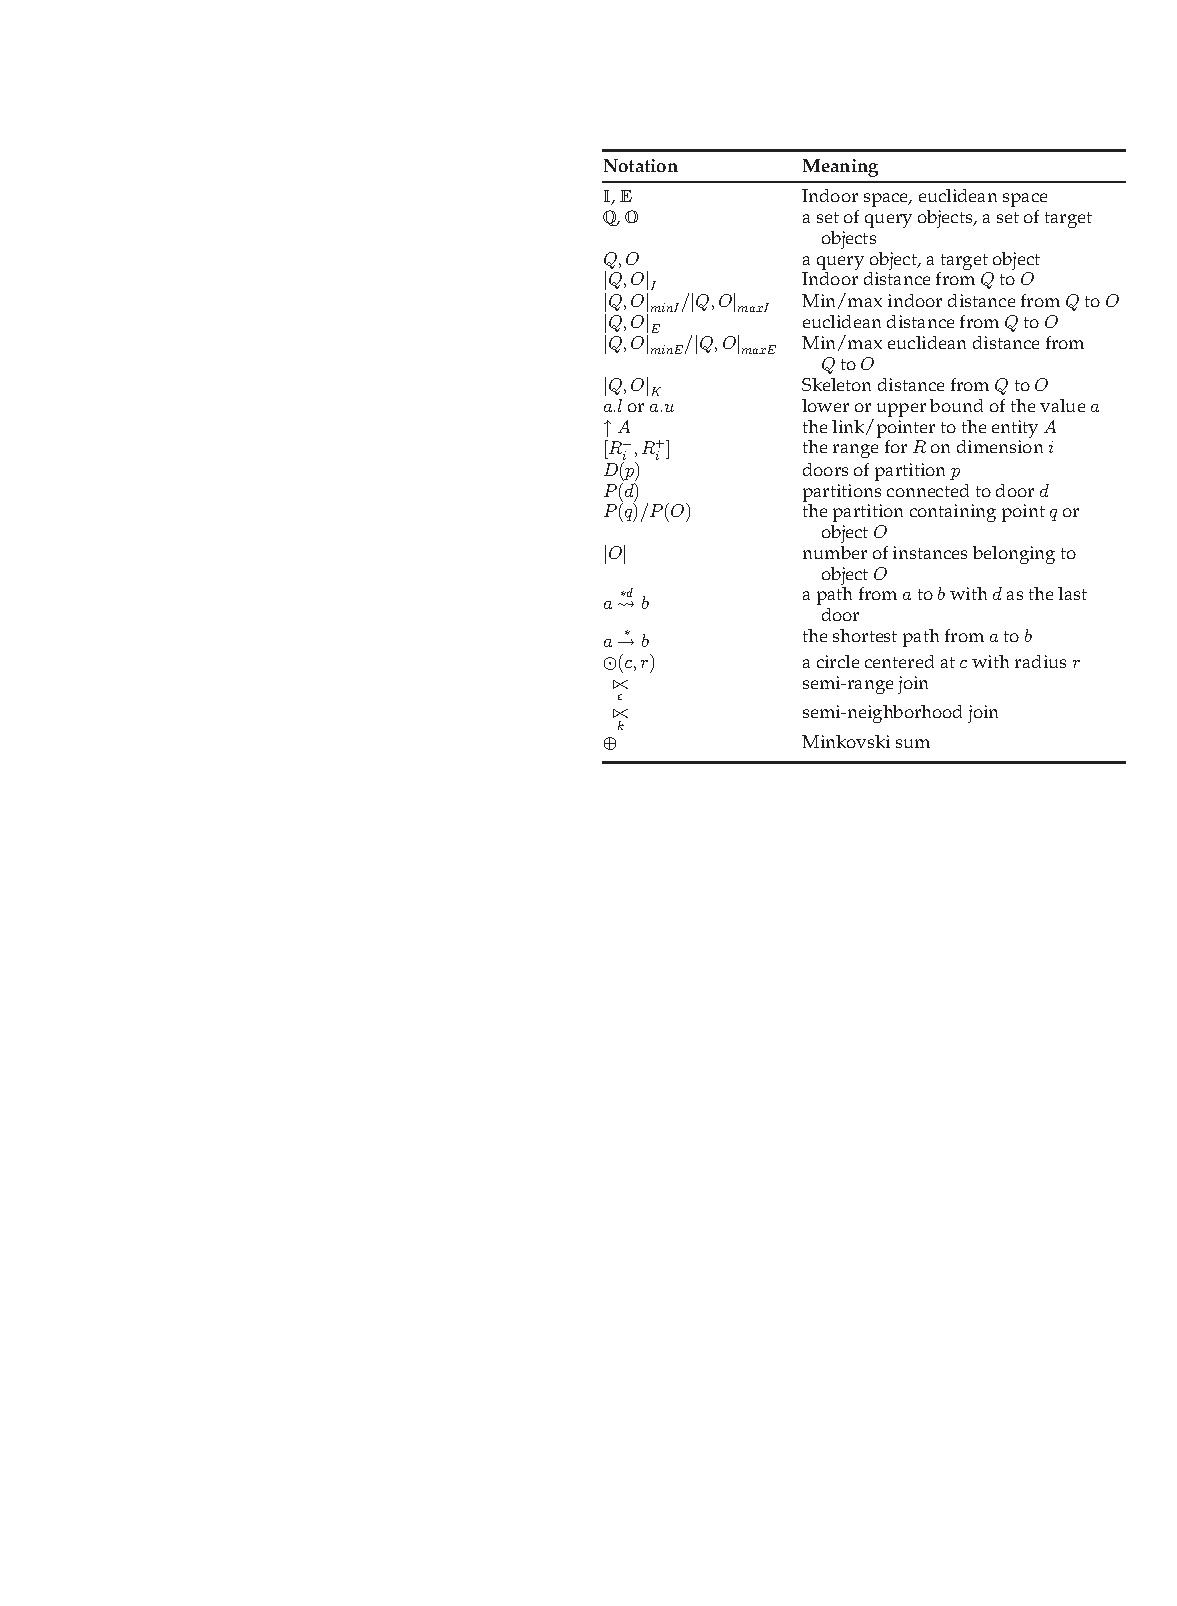
\includegraphics[width=0.57\columnwidth]{figures/2-7/2-7-1.pdf}
\end{figure}

\end{frame}

%------------------------------------------------

\begin{frame}
\frametitle{Preliminaries: Indoor Space and Indoor Distance}

\conceptbf{Doors Graph} has been proposed to represent the connectivity of indoor partitions as well as door-to-door distances.~\cite{DBLP:conf/edbt/YangLJ10}\\~\\\pause

Given two indoor positions $p$ an $q$, we use $q \overset{\delta}{\rightsquigarrow} p$ to denote a path from $q$ to $p$ where $\delta$ is the sequence of doors on the path.\\~\\\pause

The length of the shortest path as \emph{indoor distance} from $q$ to $p$, and denote it formally as $|q, p|_{I} = min_{\delta}(|q \overset{\delta}{\rightsquigarrow} p|)$, also $q \overset{\delta}{\rightarrow} p$.\\~\\\pause

\emph{indoor distance} consists of \emph{door-door distance} and \emph{intra-partition object-door distance}:\pause
\begin{equation}
  min_{d_q \in D(q), d_p \in D(p)}(|q, d_q|_{E} + |d_q, d_p|_{I} + |d_p, p|_{E})
\end{equation}

\end{frame}

%------------------------------------------------

\begin{frame}
\frametitle{Indoor Moving Objects}

\begin{itemize}
  \item Existing proposals~\cite{pfoser1999capturing, DBLP:conf/edbt/YangLJ10} model a moving object by an \emph{uncertainty region}, where the exact location is considered as a random variable inside.
  \item The possibility of its appearance can be collected by object's velocities~\cite{DBLP:conf/edbt/YangLJ10}, parameters of positioning device~\cite{pfoser1999capturing}, or analysis of historical records (represented by \emph{pdf}).
  \item The \emph{pdf} can be either a close form equation~\cite{cheng2003evaluating,cheng2004querying} or a set of instance representation~\cite{kriegel2007probabilistic}, as it is general for arbitrary distribution.
  \item Thus, an indoor moving object $O$ is represented by a set ${(o, o.\rho)}$, where $o$ is an instance and $o.\rho$ is its \emph{existential probability}, satisfying $\sum_{o \in O}o.\rho = 1$.
\end{itemize}

\end{frame}

%------------------------------------------------

\begin{frame}
\frametitle{Expected Indoor Distance}

\begin{definition}[Expected Indoor Distance for Uncertain Object]
  Given two uncertain object $Q$ and $O$, the indoor distance between $Q$ to $O$ is
  \begin{equation}
    |Q, O|_{I} = E_{q \in Q, o \in O}(|q,o|_{I}) = \sum_{q \in Q}\sum_{o \in O}|q,o|_{I} \cdot q.\rho \cdot o.\rho
  \end{equation}
\end{definition}
\vspace{10pt}
an object $O$'s uncertainty region may overlap with multiple partitions. Accordingly, all the instances in $O$ are divided into subsets, i.e., $O = \cup_{1 \leq j \leq m}O[j](1 \leq m \leq |O|)$ where each $O[j]$ corresponds to a different partition, it is called $O$'s \emph{uncertainty subregion}.

\end{frame}

%------------------------------------------------

\begin{frame}
\frametitle{Case of Indoor Distance $|Q, O|_I$ (I)}

\conceptbf{Single-Partition Single-Path Distance} \quad $O$'s uncertainty region falls into one single partition $P$, so does $Q$. Let $P_Q$ ($P_O$) be the partition containing $Q$ ($O$). For an arbitrary pair $(q, o)_{q \in Q, o \in O}$, the shortest path $q \overset{d_Q*d_O}{\rightarrow} o$ shares the same door sequence starting with $d_Q$ and ending with $d_O$, through which the path reaches $o$ from $q$.

\begin{equation}
  \begin{split}
  |Q, O|_{I} & = \sum_{q \in Q}\sum_{o \in O} (|q, d_Q|_E + |d_Q, d_O|_I + |d_O, o|_E)\cdot q.\rho \cdot o.\rho \\
             & = \sum_{q \in Q} |q, d_Q|_E + |d_Q, d_O|_I + \sum_{o \in O} |d_O, o|_E
  \end{split}
\end{equation}

\end{frame}

%------------------------------------------------

\begin{frame}
\frametitle{Case of Indoor Distance $|Q, O|_I$ (II)}

\conceptbf{Single-Partition Multi-Path Distance} \quad $O$ and $Q$'s uncertainty region still falls into one single partition $P$. However, for different instances $o_i$ and $o_j$, the shortest path $q \overset{*}{\rightarrow} o_i$ and $q \overset{*}{\rightarrow} o_j$ do not share the same door sequence.

\begin{equation}
  |Q, O|_{I} = \sum_{o_i \in O}|q, o_i|_I \cdot q.\rho \cdot o_i.\rho
\end{equation}

\begin{columns}[c]

  \column{0.24\textwidth}
  \begin{figure}[tb]
    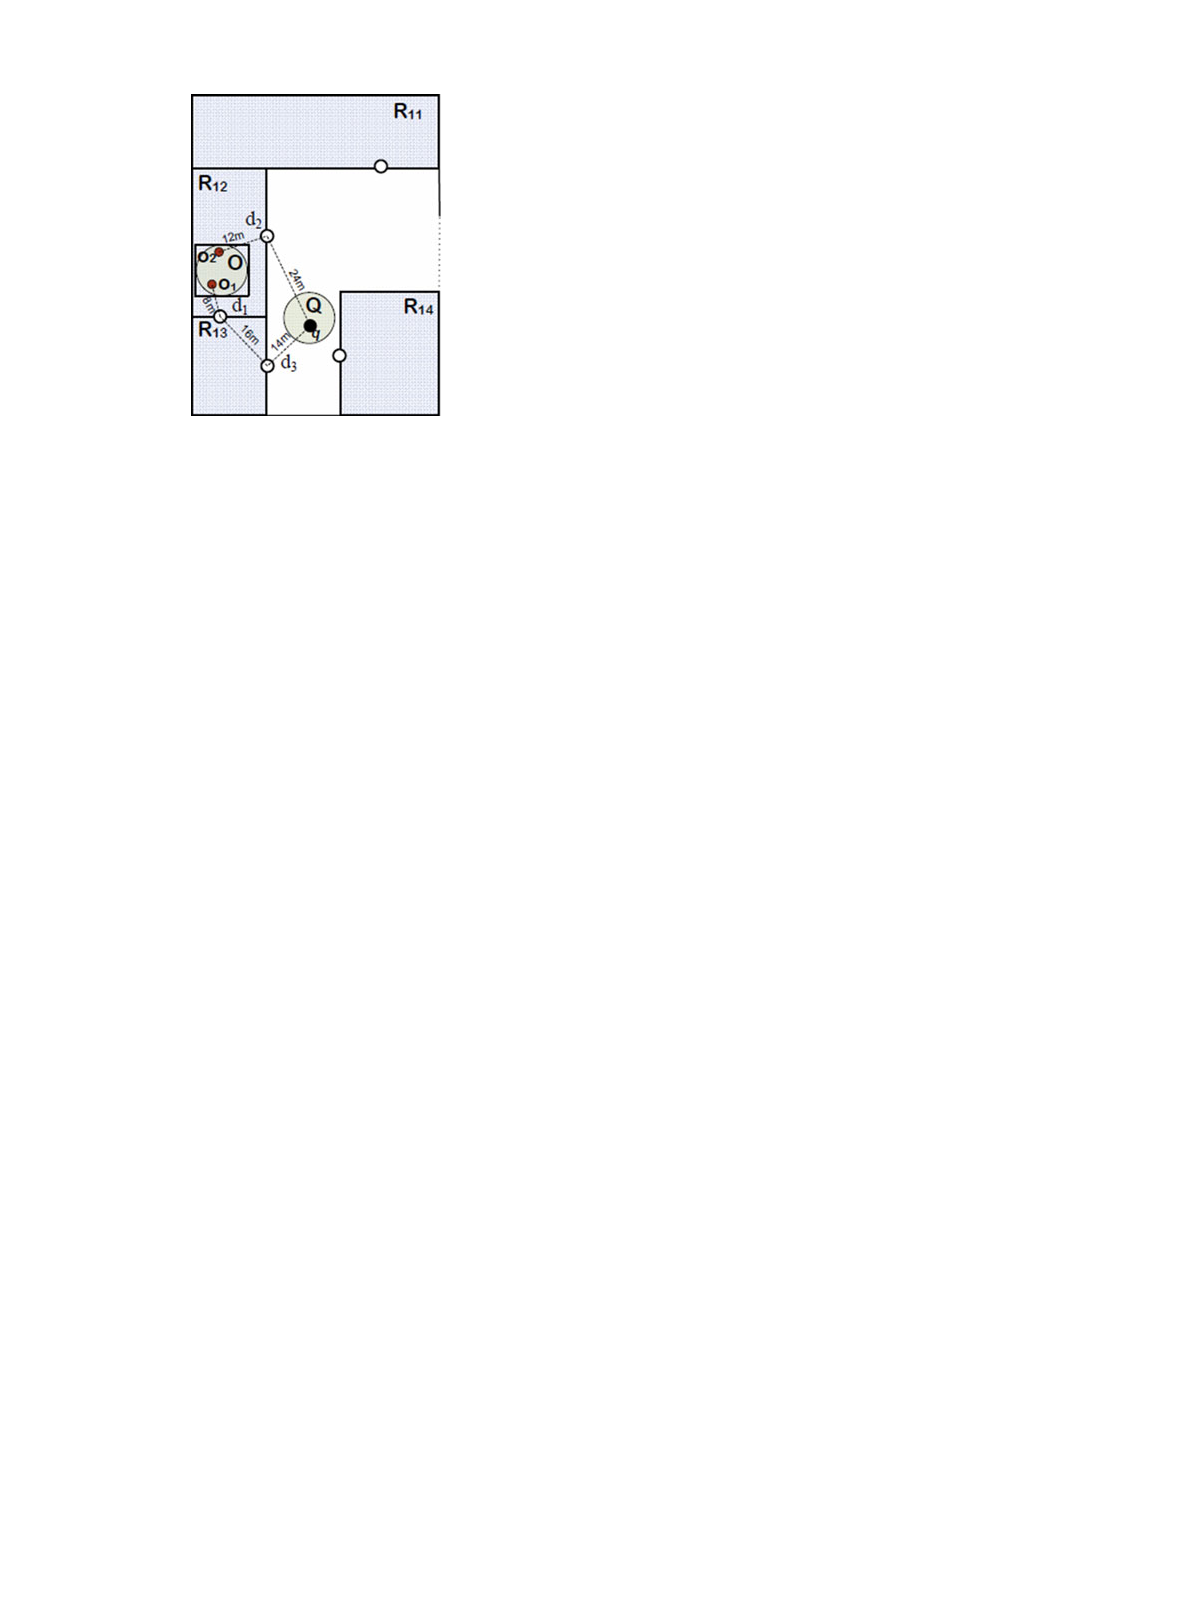
\includegraphics[width=\columnwidth]{figures/2-7/2-7-2.pdf}
  \end{figure}

  \column{0.76\textwidth}
  \begin{example}
    $O$ has two instance $o_1$ and $o_2$, the shortest path from $q$ to them are: $q \overset{d_3, d_1}{\rightsquigarrow} o_1$ and $q \overset{d_2}{\rightsquigarrow} o_2$.
  \end{example}

\end{columns}

\end{frame}

%------------------------------------------------

\begin{frame}
\frametitle{Case of Indoor Distance $|Q, O|_I$ (III)}

\conceptbf{Multi-Partition Multi-Path Distance} \quad either $Q$ or $O$'s uncertainty region overlaps with more than one partition, and thus $O = \cup_{1 \leq j \leq m}O[j](1 \leq m \leq |O|)$.

\begin{equation}
  |Q, O|_I = \sum_{i}\sum_{j}(|Q[i],O[j]|_I \cdot \sum_{q \in Q[i]}q.\rho \cdot \sum_{o \in O[j]}o.\rho)
\end{equation}

$|Q[i],O[j]|_I$ is calculated according to case I or case II.

\vspace{-5pt}
\begin{columns}[c]

  \column{0.2\textwidth}
  \begin{figure}[tb]
    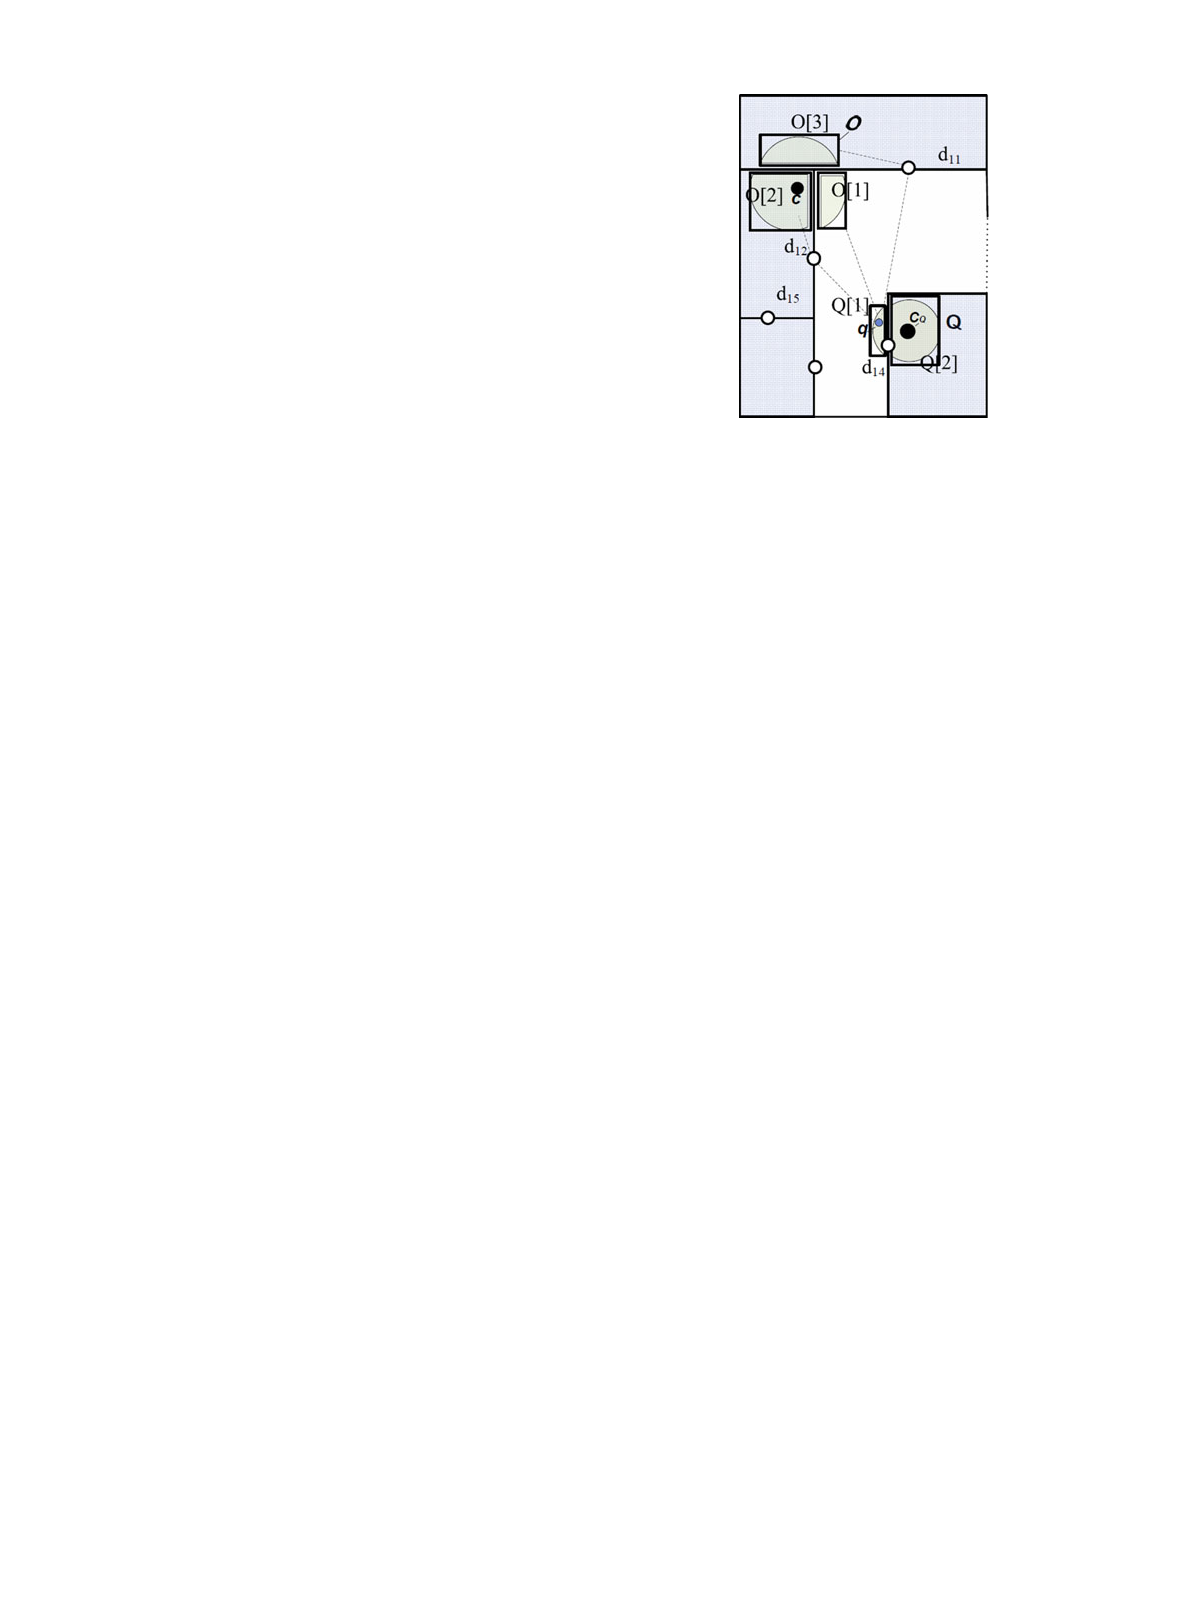
\includegraphics[width=\columnwidth]{figures/2-7/2-7-3.pdf}
  \end{figure}

  \column{0.8\textwidth}
  \begin{example}
    $O$ has three uncertainty subregions $O[1]$, $O[2]$ and $O[3]$. Accordingly, $|Q,O|_I = E(\sum_{1 \leq j \leq 3}(|q, O[j]_I|))$.
  \end{example}

\end{columns}

\end{frame}

%------------------------------------------------

\begin{frame}
\frametitle{Bounds for Indoor Distances}

\conceptbf{Geometric Layer Lower Bounds}\\
\ssize{
Fot two indoor uncertain objects $Q$ and $O$, the (virtual) euclidean distance between them is the lower bound of their distance in the indoor space. Therefore, it has $|Q,O|_{minE} \leq |Q,O|_{minI}$, where $|Q, O|_{minE} = \min_{q \in Q, o \in O}|q,o|_E$.
}

\vspace{10pt}
\begin{lemma}[Geometric Lower Bounds]
  Given indoor object $Q$ denoted by $\odot(c_Q, r_Q)$, and $O$ denoted by $\odot(c_O, r_O)$, the geomtric lower bound property can be rewritten as:
  \begin{equation}
    |c_Q, c_O|_E - r_Q - r_O \geq |Q, O|_{minI}
  \end{equation}
\end{lemma}

\vspace{10pt}
\textrm{it is impossible to derive the indoor upper bounds by using Euclidean distances only.}

\end{frame}

%------------------------------------------------

\begin{frame}
\frametitle{Bounds for Indoor Distances}

\conceptbf{Indoor Topological ULBounds}

\vspace{30pt}

For two objects $Q = \bigcup_{i = 1}^{m} Q[i]$ and $O = \bigcup_{j = 1}^{n} O[j]$, suppose that $P(Q[i])$ is the partition containing subregion $Q[i]$ and $P(Q)$ are the partitions overlapping with $Q$.

\end{frame}


%------------------------------------------------

\begin{frame}
\frametitle{Bounds for Indoor Distances}

\begin{lemma}[Topological Lower Bounds]
  \ssize{
  Let $t_{min}(Q[i], O[j])$ be: $$\min_{d_q \in D(P(Q[i])), d_s \in D(P(O[j]))}|Q[i],d_q|_{minE} + |d_q \overset{*}{\rightarrow} d_s| + |d_s, O[j]|_{minE}$$. Then, $|Q,O|_I \geq min_{i,j}\{ t_{min}(Q[i], O[j]) \}$.
  }
\end{lemma}

\begin{lemma}[Topological Upper Bounds]
  \ssize{
  Let $t_{max}(Q[i], O[j])$ be: $$\min_{d_q \in D(P(Q[i])), d_s \in D(P(O[j]))}|Q[i],d_q|_{maxE} + |d_q \overset{*}{\rightarrow} d_s| + |d_s, O[j]|_{maxE}$$. Then, $|Q,O|_I \leq max_{i,j}\{ t_{max}(Q[i], O[j]) \}$.
  }
\end{lemma}

\ssize{\textrm{Suppose $Q$ and $O$ overlap with $m$ and $n$ partitions respectively. The above two lemmas involve $O(mn)$ shortest paths.}}

\end{frame}

%------------------------------------------------

\begin{frame}
\frametitle{Bounds for Indoor Distances}

\ssize{\textrm{If $Q$ and $O$'s uncertainty regions both overlap with one partition, the above two lemmas can be rewritten.}}

\begin{lemma}[]
  \ssize{
  Given two indoor object $Q$ and $O$, denoted by $\odot(c_Q, r_Q)$ and $\odot(c_O, r_O)$ respectively, the topological ULBounds can be rewritten as:
  }
  \begin{equation}
    |c_Q, c_O|_I - r_Q - r_O \leq |Q, O|_I \leq |c_Q, c_O|_I + r_Q + r_O
    \label{equation:simplified_1}
  \end{equation}

\end{lemma}

\begin{proof}{}
  \ssize{
  \begin{equation*}
    \begin{split}
    |Q, O|_{minI} & = \min_{\forall q \in Q}(|q, O|_I) \geq \min_{\forall q \in Q}(|q, c_O|_I - r_O) = \min_{\forall q \in Q}(|q, c_O|_I) - r_O \\
    & \geq |c_Q, c_O|_I - r_Q - r_O \\
    & \Rightarrow |Q, O|_{minI} \geq |c_Q, c_O|_I - r_Q - r_O \\
    & \Rightarrow |Q, O|_{I} \geq |c_Q, c_O|_I - r_Q - r_O \\
    \end{split}
  \end{equation*}
  $|Q, O|_I \leq |c_Q, c_O|_I + r_Q + r_O$ can be proved likewise.
  }
\end{proof}

\end{frame}

%------------------------------------------------

\begin{frame}
\frametitle{Bounds for Indoor Distances}

\textrm{The shortest path $|d_q \overset{*}{\rightarrow} d_s|$ computation is not economic, a \conceptbf{Topological Looser UBound} is proposed. }

\begin{lemma}[Topological Looser Upper Bounds]
  \ssize{
  Let $t_{max}(Q[i], O[j])$ be: $$\min_{d_q \in D(P(Q[i])), d_s \in D(P(O[j]))}|Q[i],d_q|_{maxE} + |d_q \overset{*}{\rightsquigarrow} d_s| + |d_s, O[j]|_{maxE}$$. Then, $|Q,O|_I \leq max_{i,j}\{ t_{max}(Q[i], O[j]) \}$.
  }
\end{lemma}

\textrm{In the case that both $Q$ and $O$ overlap with one partition, the lemma can be simplified as:}
\begin{equation}
  \min_{d_q \in D(P(Q[i])), d_s \in D(P(O[j]))} |d_q \overset{*}{\rightsquigarrow} d_s| + |d_q, c_Q|_E + |d_o, c_O|_E + r_Q + r_O
  \label{equation:simplified_2}
\end{equation}

\end{frame}

%------------------------------------------------

\begin{frame}
\frametitle{Bounds for Indoor Distances}

\fsize{
The simplified versions of ULBounds are more efficient since they only take one shortest path instead of $O(mn)$ paths. To generalize the single-parition case to multiple-partition scenarios, \conceptbf{star-connected region} is defined.
}

\begin{definition}[Star-connected regions]

  Let $O = \odot(c, r)$ be an indoor object overlapping with more than one partition, i.e., $O = \bigcup_{i=1}^{n}O[i]$. Let the subregion containing $c$ be the central region $C$. If all other subregions are connected to $C$ by doors, we call $O$'s region a star-connected region, formally:

  \begin{equation*}
    \forall O[i] \neq C, \exists~\text{door}~d , \text{such that}~d \in C~\text{and}~d \in O[i]
  \end{equation*}

\end{definition}


\end{frame}

%------------------------------------------------

\begin{frame}
\frametitle{Bounds for Indoor Distances}

\begin{columns}[c]

  \column{0.2\textwidth}
  \begin{figure}[tb]
    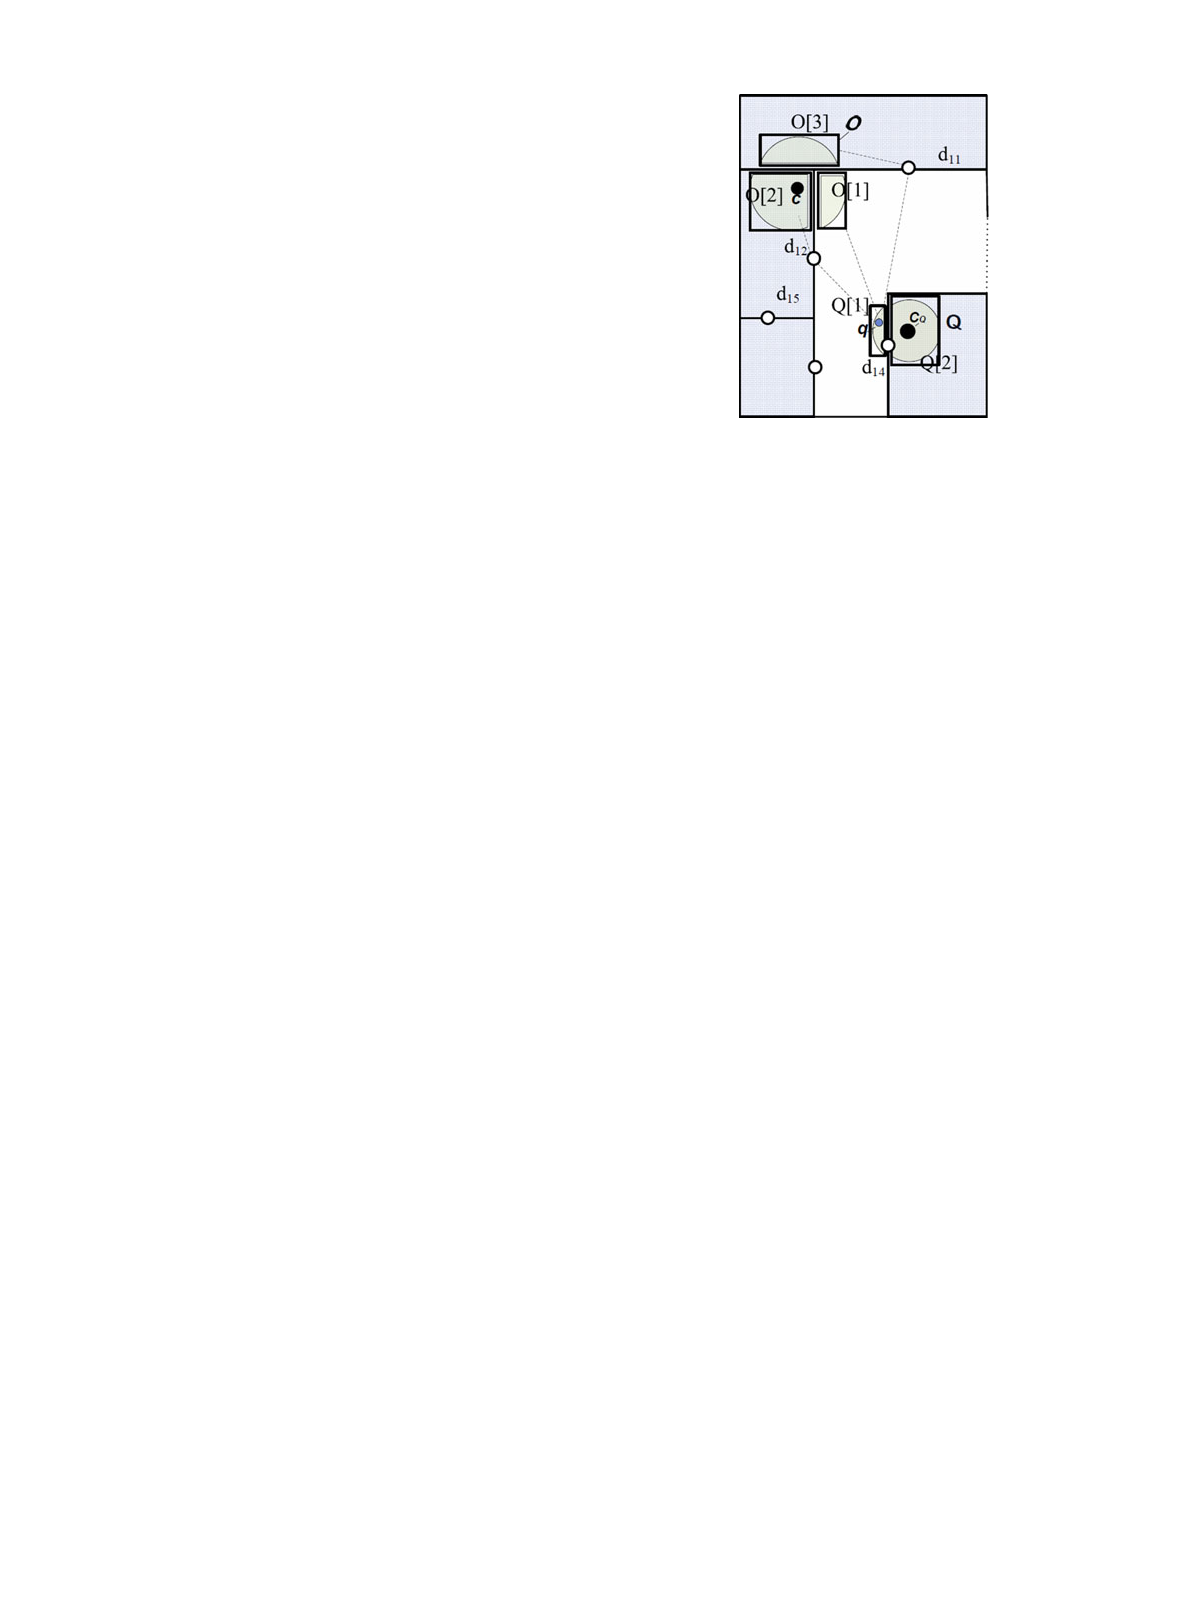
\includegraphics[width=\columnwidth]{figures/2-7/2-7-3.pdf}
  \end{figure}

  \column{0.8\textwidth}
  \begin{example}
    \ssize{
    $Q$ is a star-connected region, since $Q[1]$ and $Q[2]$ are connected by door $d_{14}$, $O$ is not a star-connected region, since $O[2]$ and $O[3]$ are separated into two partitions, and there is no door connecting the two partitions.
    }
  \end{example}

\end{columns}

\vspace{10pt}

\textrm{Then, we can define $O$ by $\odot(c, r_I)$, where $r_I$ is the maximum indoor distance from centroid $c$ to all subregions, $r_I = \max_{i} |c, O[i]|_{maxI}$. By defining star-connected regions, we can benefit from the simplifications in topological ULBounds by substituting $r_I$ into Equations.(\ref{equation:simplified_1}), (\ref{equation:simplified_2}).}

\end{frame}

%------------------------------------------------

\begin{frame}
\frametitle{Bounds for Indoor Distances}

\begin{columns}[c]

  \column{0.2\textwidth}
  \begin{figure}[tb]
    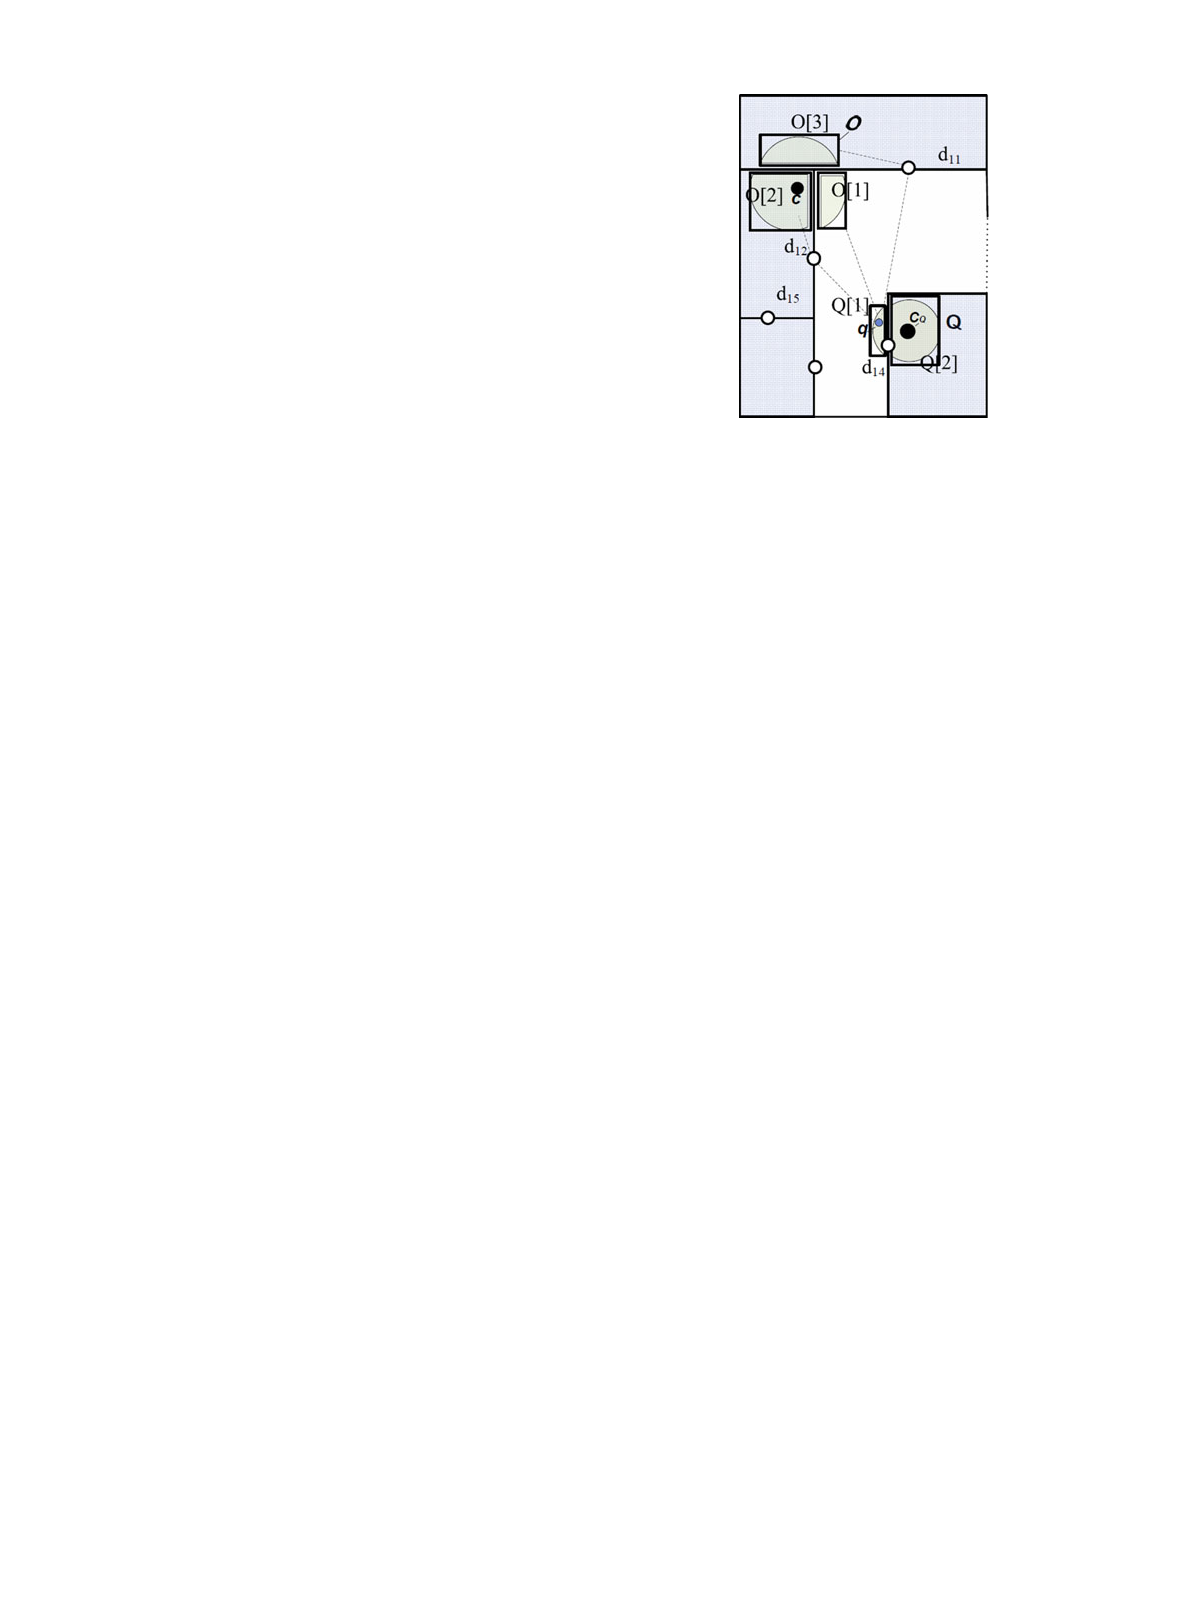
\includegraphics[width=\columnwidth]{figures/2-7/2-7-3.pdf}
  \end{figure}

  \column{0.8\textwidth}
  \begin{example}
    \ssize{
    the distance from $q$ to $O[1]$ is short, while the distance to $O[3]$ is long. If the gap between topological upper and lower bounds is large, the expected distance is only constrained by a loose range and thus not well approximated.
    }
  \end{example}

\end{columns}

\vspace{15pt}

\textrm{Geometric and topological ULBounds bound the distance by the minimum/maximum distance between sample pairs. The \conceptbf{Object Layer ULBounds} make a difference by considering the probability distributions among sample points.}

\end{frame}
